%}).\section{Background and Motivation}
%\label{motivation}
%
%\begin{figure}[t]
%\centering
%\includegraphics[width=1.0\columnwidth]{thermostat/figures/hotspot-cdf.png}
%\caption{HotSpot huge page distribution}
%\vspace{-0.175in}
%\label{fig:hotspot-cdf}
%\end{figure}
%
%Cold data at 4KB granularity vs 2MB granularity. Use figure to show quantify
%HotSpot pages within an otherwise cold huge page.
%
%Show analytical analysis of putting pages in slow memory and opportunity to make
%slow memory usable in data centers.
%
%Discuss performance-cost trade-off for data centers.
%
%Why are previous 2-level memory techniques inadeqaute in solving this issue.
%
%Re-iterate the problem we are solving and the central idea of our solution.
%
\section{Background}
\subsection{Virtual Memory Management}
\begin{figure}[t]
\centering
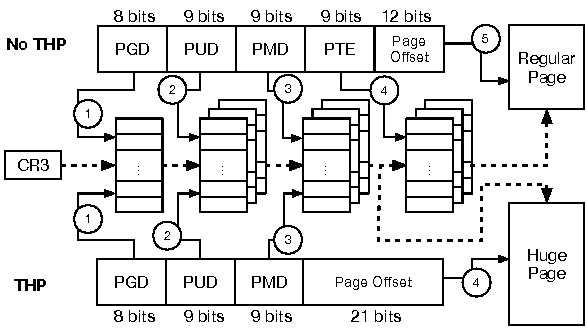
\includegraphics[width=0.45\textwidth]{thermostat/figures/linux_pgtable.pdf}
\caption{
Linux page table structure for X86 both with and without a transparent huge page.
}
\label{fig:linuxpgtable}
\end{figure}


As the size of main memory has grown, the overheads of virtual memory systems
have grown as well.  The hierarchical Linux page table for the x86-64
architecture, shown in Figure~\ref{fig:linuxpgtable}, 
is four levels -- and thus may incur up to four extra main memory
accesses to walk the page table in~\cite{pgtable}.
%\fixme{This text is a candidate to cut to save space: Translation begins with
%the page global directory (PGD), pointed to by the CR3 register, which is
%preloaded with the PGD base address upon a context switch.  Bits 39-46 of the
%virtual address are used to index the PGD, yielding a page upper directory
%(PUD) structure, which is subsequently indexed by bits 30-38 of the virtual
%address to produce a page middle directory (PMD) structure.  When the
%translation target lies on a physical page of the 4 KB base page size (shown on
%the top in \pref{fig:linuxpgtable}), the PMD is indexed with bits 21-29, giving
%a page table entry (PTE) that is indexed by bits 12-20 to finally generate a
%physical page number.  Throughout this process, as many as four extra memory
%operations may be performed purely as an overhead of the virtual memory
%translation system.}
Moreover, execution in virtualized environments can increase number of memory
accesses to 24, a $6x$ increase from the non-virtualized case 
\cite{amdnested,intelept,bhargava:2008:atp}.  As a result, the Translation
Lookaside Buffer (TLB), which acts as a cache for virtual-to-physical mappings,
has become increasingly important to mollify the effects of virtual memory
translation overhead.

In most architectures, TLB accesses lie on the critical path of memory accesses,
hence hardware timing constraints limit the number of TLB entries that can be
searched on each access.  As memory capacities grow while page sizes remain
constant, TLB coverage -- the fraction of main memory that can be represented by
the contents of the TLB at any given time -- necessarily decreases.  This reduced
coverage hampers the performance of programs with large working sets and/or
instruction footprints because it increases the number of TLB misses they
exhibit, and thus the number of page table walks that must be performed.  What's
more, as working set sizes -- and, correspondingly, page table sizes -- grow, the
fraction of translation data that can fit in the cache is reduced, leading to
more severe TLB miss penalties.

%Recognizing the high cost of TLB misses in cloud applications, a number of
%recent research efforts have sought hardware solutions to mitigate their penalty
%(e.g., \cite{bhattacharjee:2011:slt, srikantaiah:2010:sth, barr:2011:sms,
%pham:2012:ccl, basu:2013:evm, gandhi:2014:emv}).
%Whereas these techniques reduce or hide TLB miss stalls, they do not address the
%cost of managing numerous page tables entries or the cache capacity occupied by
%them.
%
%One line of work seeks architectural solutions to improve the reach of TLBs,
%for example, through 2-level TLBs .  These mechanisms can improve TLB hit
%rates, but require hardware changes and do not address the cost of managing
%page tables, which manifest during a variety of system calls (e.g., upon
%allocations, faults to access \texttt{mmap()}'d files, and forks).  A second
%line of work revisits alternative memory virtualization schemes, such as
%segmentation, in the context of modern systems \cite{basu:2013:evm,
%gandhi:2014:emv}.  While new hardware support for segmentation may address TLB
%capacity limitations for the user heap, it does not provide a straightforward
%solution for OS structures that may require finer-grained protection, such as
%the file system page cache.

Huge pages directly address the costs of fine-grain page management.
%They require hardware support in the TLB for huge-page entries (either
%dedicated entries or support for multiple-sized lookups), but this support is
%ubiquitous in existing architectures (e.g., Intel's Haswell processor
%provisions 32 entries for huge pages in its L1 data TLBs).
They effectively increase TLB coverage -- one huge page TLB entry covers the area
of a large number of regular page entries -- thus reducing page faults, and they
reduce the size of the page table structure, leading to both fewer memory
accesses upon a TLB miss and increased cache-ability of translation data.
%on a TLB miss they can reduce the number of page table accesses necessary to
%resolve a virtual-to-physical mapping.  The latter arises due to the fact that
%a huge page covers a much larger range of virtual memory.
%\pref{fig:ahppgtable} displays the most efficient possible hierarchical page
%table topology for x86-64 Linux if it is backed by 2MB huge pages.
%In contrast to the page table shown in \pref{fig:linuxpgtable}, this structure
%requires only two extra memory accesses due to the increased coverage at each
%level.  Though TLB support for huge pages is ubiquitous in existing
%architectures (e.g., Intel's Haswell processor TLBs provision 32 entries for
%huge pages in the L1 data TLB), unfortunately the current x86-64 architecture
%specifies the page table layouts shown in \pref{fig:linuxpgtable}.
%and precludes a design like that in \pref{fig:ahppgtable}.
%We hope our results might motivate greater flexibility in future architecture
%revisions.
%
%\input{fig.ahppgtable}

\subsection{Transparent Huge Pages} \label{sec:thp_bg}
%\fixme{This paragraph strongly duplicates the intro.  We should say this in
%only one place.  My suggestion is to cut down the intro and leave the details
%here. --- Jeff: fixed}
Early system support for huge pages, static huge pages, requires bucketing the
available physical memory at boot time into standard pages and huge pages.
Static huge pages are disjoint from the standard memory pool and cannot be used
for the disk page cache, disk write buffers, or any kernel data structure.
Moreover static huge pages require application changes and are thus
non-transparent to the programmer. The static provisioning of memory into static
huge pages also leads to allocation problems and memory stranding if the actual
demand for huge pages does not match the boot-time configuration.  Thus, even if
applications are static huge page-aware, such a solution is less than ideal for
many systems because it requires a priori knowledge of applications' memory
requirements to ensure ideal performance.

Recent versions of the Linux kernel instead exploit huge pages through THP.
With THP, the kernel attempts to invisibly (i.e., without the knowledge of the
user) allocate huge pages to back large regions of contiguous virtual memory.
Transparent allocation is advantageous because it allows existing code bases to
reap the rewards of huge pages without modification and doesn't require changing
the interfaces and invariants of system calls and functions that require
consideration of page size, such as \texttt{mmap()}.  However, the kernel may
demote allocated huge pages by breaking them down into a set of regular pages
when it deems necessary  to maintain support for functions that are not huge
page-aware.

\textbf{Allocation/Promotion:} The first time an application touches an
allocated region of virtual memory, a page fault occurs and the kernel allocates
one or more physical pages to back that region and records the virtual to
physical mapping.  With THP enabled, the kernel allocates huge pages for
anonymous (i.e., non-file-backed) regions of huge page-sized and -aligned
virtually contiguous memory during the initial page fault to that region.
%Alternatively, if a huge page isn't initially available or the size and
%alignment requirements are not met, a region of virtual memory that isn't
%initially backed by huge pages can later be promoted if the virtual region is
%later modified to meet these requirements.  In the process of promotion, the
%regular page-backed virtual region is collapsed into a huge page-backed region,
%thus multiple regular pages are marked to be treated as a single huge page.
Alternatively, if a region isn't initially backed by a huge page, it can later
undergo promotion, in which multiple regular pages are marked to be treated as a
single huge page.  The kernel can be set to either aggressively allocate huge
pages whenever it can, or to only allocate them when the user provides hints via
the \texttt{madvise()} system call.

\textbf{Demotion:} Any region backed by a huge page may be subject to
spontaneous demotion to regular pages.  Because various parts of the kernel
source code are not huge page-aware, giving them access to a huge page could
lead to unspecified or erroneous behavior.  As a result, huge pages are often
\emph{split}, or broken into several regular pages, before they are passed to
functions that are not huge page-aware.  To perform this split, the page table
must be updated to reflect the many regular pages that comprise the demoted huge
page.

%Another notable characteristic of THP is that it does not increase the coverage
%of the various levels of the page table (due to architectural constraints
%described in \pref{sec:limitations}).  Therefore, while the physical page size
%is increased, the coverage of each level of the page table remains the same.
%The translation procedure for \thp, shown on the bottom in
%\pref{fig:linuxpgtable}, elides the PMD$\to$PTE step necessary with regular
%pages and produces a physical page number at the PMD level.
%
%In contrast to the two memory access translation shown in
%\pref{fig:ahppgtable}, a \thp translation requires three accesses.
%
%\subsection{Pathologies of THP} \label{sec:thp_problems}
%
%\input{fig.frag_bench.tex}
%
%Though \thp has the potential to improve average application throughput, it can
%negatively impact latency and performance isolation between unrelated
%applications.  A widely known effect of paged virtual memory is external memory
%fragmentation---small blocks of free memory separated by large blocks of
%allocated memory.  With \thp, a system exhibiting significant memory
%fragmentation may not always have huge page-sized regions of contiguous
%physical memory available for allocation, even if much of memory is free.
%
%Severe memory fragmentation is particularly common in cloud computing
%workloads, where processes start and end frequently.  In systems with few,
%long-lived processes, virtual memory rarely becomes fragmented---most user-mode
%allocators do not frequently return freed memory to the operating system,
%instead retaining and managing it in pools.  In contrast, many cloud
%environments collocate multiple processes that start and end frequently in a
%single machine.  For example, map-reduce clusters execute thousands of
%processes that may each last only minutes.  Main memory will rapidly fragment
%due to the varying allocation sizes of these numerous short-lived processes.
%I/O intensive workloads can also cause rapid memory fragmentation due to random
%access I/O populating the page cache with many small allocations, which are
%subsequently reclaimed without regard to layout.
%
%When a huge page is requested during a page fault but cannot be served, the
%Linux memory manager has two options: it can either turn down the request and
%fall back on regular pages to serve the fault, or it can stall the program and
%defragment memory to create a huge page-sized chunk to allocate.  The former
%option is not ideal, as it prevents applications from reaping the benefits of
%huge pages when there is still enough physical memory available to accommodate
%them.  However, the performance cost of synchronous (\ie, blocking)
%defragmentation can be significant, as execution of the application must be
%paused while the kernel migrates regular pages to make room for a huge page.
%
%While defragmentation is in progress, the kernel will obtain and hold locks
%that can block progress of other applications that happen to concurrently
%request memory.  Hence, defragmentation impacts not only the application
%requesting the huge page, it can also result in stalls in ``innocent
%bystander'' applications.  Indeed, in our experience, a pathological behavior
%in defragmentation code triggered by one application caused multi-millisecond
%(and initially unexplainable) latency spikes in an unrelated production service
%that happened to collocate on the same server.  The kernel locks held by
%defragmentation code caused allocation delays to spread virally among
%applications.  These THP pathologies have been documented by others as well
%\cite{zhuang:2014:ehm, rientjes:2014:email, oracle:2013:blog, rahn:2012:blog}.
%Whereas some of these issues have been mitigated (after several man-months of
%investigation), these pathologies motivated this study of the \thp mechanism,
%and prompted us to ask whether, perhaps, the entire mechanism should be
%discarded.
%
%To our dismay, one such pathology in \thp can be triggered in recent versions
%of the kernel (in which the behavior is ostensibly fixed), even without exotic
%application behaviors.  To reconstruct this behavior, we use a memory
%allocation microbenchmark that measures the latency of allocation (\ie, time
%needed for the kernel to find and map a physical page) for 2MB regions
%allocated on the heap using unmodified GLIBC \texttt{malloc()}.
%\pref{fig:frag_bench} shows the impact of synchronous memory defragmentation on
%allocation tail latency in a virtual machine running version 3.13 of the Linux
%kernel.
%% when using only \texttt{malloc()} to fragment memory, as might naturally arise after running map-reduce processes for several hours. %
%%We measure a memory allocation microbenchmark, which allocates and initializes huge page-sized chunks of memory using unmodified GLIBC \texttt{malloc()}, causing the kernel to attempt to allocate huge pages when the THP mechanism is enabled.
%We report the cumulative distribution of the latency of individual allocations
%(note the logarithmic x-axis scale).  We consider four scenarios, two with \thp
%enabled and two with it disabled.  We consider scenarios where memory is
%initially unfragmented (all memory is free and the page cache is empty) and
%where it has been aggressively fragmented.  We fragment memory using a large
%number of processes that repeatedly allocate and free memory chunks of random
%sizes---a scenario representative of a series of map-reduce tasks.  These
%processes are continually spawned and killed (to return their allocated memory
%to the kernel), with the last set of processes ultimately holding a final set
%of allocations (partially filling memory) and quiescing.  Further details of
%our test setup appear in \pref{sec:methodology}. %\fixme{Confirm that we
%actually do provide further details in the results section.}
%
%There are two key take-aways from this experiment.  First, \thp substantially
%reduces latency for most allocations.  Median allocation latency is reduced
%from about 700us to about 500us.  Allocations become faster on average because
%the kernel must create and map far fewer PTEs (by as much as a factor of 512)
%for large allocations.  When memory is unfragmented, nearly all allocations are
%faster under \thp.  In contrast, when memory is fragmented, synchronous
%compaction severely delays a significant fraction of allocations, in some cases
%increasing latency by orders of magnitude.  About 20\% of allocation requests
%take longer than 1ms with allocations in the 99th percentile taking over 100ms.
%
%Though the tail latency of memory allocation under such circumstances isn't
%critical in all applications, especially those with steady-state heap activity,
%it can have negative effects on other tail-latency-sensitive workloads.
%Workloads such as web search, for instance, perform significant fan-out and
%fan-in operations, where stragglers impact overall latency
%\cite{dean:2013:tas}.  For such applications, unpredictable allocation tail
%latency or stalls of bystander applications/threads can severely impact
%application service level objectives.
%
%One alternative to avoid this unpredictability is to asynchronously (\ie, on
%idle cores) defragment memory to help alleviate the amount of defragmentation
%that must be done at allocation time.  This feature is available in the Linux
%kernel, but it comes with a tradeoff: setting the defragmentation daemon to be
%too aggressive causes it to consume substantial CPU time, harming the
%performance of other threads (and reducing the throughput benefit of \thp)
%\cite{zhuang:2014:ehm}, but setting it to be too passive results in little net
%benefit.  We examine this trade-off in \pref{sec:case_study}.  Alternatively,
%one might reduce the aggressiveness of or disable synchronous compaction
%altogether.  However, doing so often precludes huge page allocation, resulting
%in a performance loss in the common cases where synchronous defragmentation
%does not dominate allocation time.  Thus, supporting multiple pages sizes leads
%to a catch-22; aggressive compaction leads to performance loss due to invasive
%use of system resources, and less aggressive or no compaction results in
%performance loss because huge pages cannot always be allocated on-demand.  As a
%result, THP---or any system that supports multiple page sizes---is inherently
%disadvantaged when large chunks of memory are scarce, as when the system is
%under heavy memory pressure or subject to external fragmentation.
%%
%%under memory pressure or fragmentation.
